\documentclass[12pt,a4paper]{article}

\usepackage[slovak]{babel}
\usepackage[utf8]{inputenc}
\usepackage[T1]{fontenc}

\usepackage{float}
\usepackage{listings}
\usepackage{graphicx}
\usepackage{tabularx} 

\usepackage{hyperref} 

\usepackage{amsmath} 

\lstset{
language=sh
,breaklines=true
,basicstyle=\ttfamily
, showstringspaces=false}

\author{Peter Csiba}
\textwidth 6.5in
\oddsidemargin 0.0in
\evensidemargin 0.0in

\title{Pánko Herkules vs. Motač Hydra}
\date{12-04-2014}
\author{Peter Csiba, petherz@gmail.com}

\begin{document}
\maketitle

\section*{Abstrakt}
Začalo sa to nevinne. Trošku božia Hera, sestra a manželka Bleskofúzora nahnevalkala nášho Pánka Herkulesa. Ten vo svojom amoku zabil svoju fajnú manželku a šesť synov. "Pipkoš", povedal si Herkules, "Odteraz si budem už len motkať". Následne mu kráľ Eurystheus naložil 12 úloh, a ak ich splní, tak bude zase Pánkom uznaným samotným Bleskofúzorom. 

Druhou úlohou bolo zabiť Motač Hydru. Hydra je zakorenená strom, ktorá má listy=hlavy. Po odseknutí ľubovoľnej hlavy vyrastú nové dva pod-stromy z jej krku=nelistového vrcholu. Takže jak Herkules sečká, tak Hydre rastenkajú hlavy. Vie Herkules zabiť Hydru? Dokážte alebo vyvráťte. Budeme prezentovať dve riešenia. Jedným je brute-force Herkulesove a druhé pochill Goodsteinove z roku 1944. 

\begin{figure}[H]
\centering
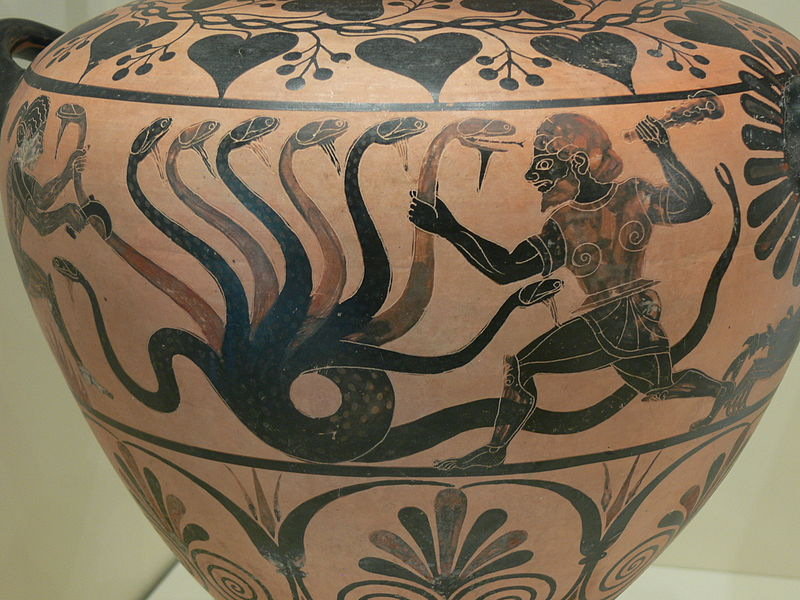
\includegraphics[width=0.6\textwidth]{hydra.png}
\end{figure} 

\section*{Prednáška}


\section*{Zdroje} 
\begin{itemize} 
\item \href{http://www.quora.com/Mathematics/What-are-some-of-the-most-counterintuitive-mathematical-results/answer/Michal-Fori\%C5\%A1ek?ref=fb}{Pôvodná inšpirácia}
\item \href{http://en.wikipedia.org/wiki/Lernaean_Hydra}{Abstrakt = Príbeh}  
\item \href{http://en.wikipedia.org/wiki/Ordinal_number}{Ordinálne čísla}
\item \href{http://en.wikipedia.org/wiki/Goodstein's_theorem}{Dôkaz}
\item \href{http://www.madore.org/~david/math/hydra.xhtml}{Applet 1 (by David A. Madore)} 
\item \href{http://math.andrej.com/wp-content/uploads/2008/02/Hydra/hydraApplet.html}{Applet 2 (by Andrej Bauer)} Idealne stiahnut .jar a prikaz: 
\begin{lstlisting}
java -cp hydra.jar hydra.HydraWindow
\end{lstlisting}
\end{itemize} 

\end{document}

